\documentclass[11pt,a4paper]{article}

% ── Fonts (clean academic) ──
\usepackage[utf8]{inputenc}
\usepackage[T1]{fontenc}
\usepackage{newtxtext,newtxmath}          % Times-based (academic standard)
\usepackage[scaled=0.85]{beramono}        % Monospace

% ── Layout ──
\usepackage[margin=2.5cm,top=3cm,bottom=2.5cm]{geometry}
\usepackage[skip=0.8em plus 2pt]{parskip}
\usepackage{microtype}
\usepackage{titlesec}
\usepackage[shortlabels]{enumitem}
\usepackage{setspace}
\setstretch{1.2}
\usepackage{lastpage}

% ── Graphics & Tables ──
\usepackage{graphicx}
\usepackage{booktabs}
\usepackage{tabularx}
\usepackage{array}
\usepackage{colortbl}
\usepackage{xcolor}
\usepackage{tikz}
\usetikzlibrary{calc}

% ── Links ──
\usepackage{hyperref}
\hypersetup{
  colorlinks=true,
  linkcolor={blue!50!black},
  urlcolor={blue!50!black},
  pdfauthor={Radical Concepts},
  pdftitle={Sprint Review — Deliverable 2},
}

% ── Minimal color palette ──
\definecolor{primary}{HTML}{111111}
\definecolor{accent}{HTML}{333333}
\definecolor{linkblue}{HTML}{1a5276}
\definecolor{muted}{HTML}{888888}
\definecolor{textmain}{HTML}{222222}
\definecolor{textsec}{HTML}{444444}
\definecolor{border}{HTML}{CCCCCC}
\definecolor{lightgray}{HTML}{F5F5F5}
\definecolor{purpleborder}{HTML}{666666}
\definecolor{greenborder}{HTML}{666666}
\definecolor{amberborder}{HTML}{666666}

\color{textmain}

% ── Section styling (academic) ──
\titleformat{\section}
  {\large\bfseries}
  {\thesection.}{0.5em}{}
\titlespacing{\section}{0pt}{1.5em}{0.5em}

\titleformat{\subsection}
  {\normalsize\bfseries}
  {\thesubsection}{0.5em}{}
\titlespacing{\subsection}{0pt}{1em}{0.3em}

\titleformat{\subsubsection}
  {\normalsize\itshape}
  {}{0em}{}
\titlespacing{\subsubsection}{0pt}{0.8em}{0.2em}

% ── Simple boxes (minimal) ──
\usepackage{tcolorbox}
\tcbuselibrary{skins,breakable}

\newtcolorbox{pivotcard}[1]{
  enhanced,breakable,
  colback=white,colframe=black!20,
  boxrule=0.4pt,arc=0pt,
  left=10pt,right=10pt,top=8pt,bottom=8pt,
  before upper={\textbf{#1}\par\smallskip},
  after skip=6pt
}

\newtcolorbox{insightcard}{
  enhanced,breakable,
  colback=lightgray,colframe=lightgray,
  boxrule=0pt,arc=0pt,
  left=10pt,right=10pt,top=8pt,bottom=8pt,
  after skip=6pt
}

\newtcolorbox{feedbackcard}{
  enhanced,breakable,
  colback=white,colframe=black!20,
  boxrule=0.4pt,arc=0pt,
  left=10pt,right=10pt,top=8pt,bottom=8pt,
  after skip=6pt
}

\newtcolorbox{toolscard}{
  enhanced,breakable,
  colback=lightgray,colframe=lightgray,
  boxrule=0pt,arc=0pt,
  left=10pt,right=10pt,top=8pt,bottom=8pt,
  after skip=6pt
}

\newtcolorbox{metriccard}{
  enhanced,
  colback=lightgray,colframe=border,
  boxrule=0.4pt,arc=0pt,
  left=10pt,right=10pt,top=8pt,bottom=8pt,
}

% ── Header/Footer ──
\usepackage{fancyhdr}
\pagestyle{fancy}
\fancyhf{}
\fancyhead[L]{\small Radical Concepts --- Sprint Review}
\fancyhead[R]{\small Deliverable \#2}
\fancyfoot[C]{\small\thepage}
\renewcommand{\headrulewidth}{0.4pt}
\renewcommand{\footrulewidth}{0pt}

% ── Lists ──
\setlist[itemize]{nosep,left=0pt..1.5em}
\setlist[enumerate]{nosep,left=0pt..1.5em}

% ── Inline tag (grayscale) ──
\newcommand{\ptag}[2]{%
  \tikz[baseline=(t.base)]{%
    \node[fill=black!75,text=white,font=\footnotesize\bfseries,
          inner xsep=4pt,inner ysep=1.5pt,rounded corners=1.5pt] (t) {\uppercase{#2}};%
  }%
}

% ── Link ──
\newcommand{\linkto}[2]{\href{#1}{#2}}

\begin{document}

% ═══════════════════════════════════════
% TITLE
% ═══════════════════════════════════════
\thispagestyle{plain}

\begin{center}
  {\LARGE\bfseries Sprint Review --- Deliverable \#2}\\[0.8em]
  {\large Fasten Your Seatbelt: Politics, Tech \& Interesting Stuff}\\[0.3em]
  {\normalsize An end-to-end AI podcast pipeline for Brett Moore}\\[2em]
  \begin{tabular}{rl}
    \textbf{Team:} & Radical Concepts --- Chris, Kalina, Roxy, Angelo, Hamid \\
    \textbf{Client:} & Brett Moore, Barcelona \\
    \textbf{Sprint:} & 1 (Feb 24 -- Mar 14, 2026) \\
    \textbf{Course:} & Innovation to Practice (I2P), ESADE \\
    \textbf{Mentor:} & Farid \\
    \textbf{Date:} & March 17, 2026 \\
  \end{tabular}
\end{center}

\vspace{1em}
\hrule
\vspace{1em}

% ═══════════════════════════════════════
\section{Product Increment}
% ═══════════════════════════════════════

\subsection{Direction}

We presented 3 concept pitches to Brett (Deliverable \#1): \emph{Automated Political Podcast}, \emph{The Curiosity Game}, and \emph{The Dinner Table Drop}. Rather than picking one, Brett asked us to go deeper---to \textbf{refine his original podcast concept} using our research insights. This led us to modularize the entire podcast production workflow into stages and modules, and to explore what an end-to-end AI pipeline could look like for him.

\subsection{What We Did}

\subsubsection{System Architecture}

We first identified the overall stages and modules of the pipeline. The architecture consists of 4 stages with 7 modules (\linkto{https://b1rd33.github.io/radical-concepts-context/pipeline.html}{Interactive Pipeline Builder}):

\vspace{0.8em}
\begin{center}
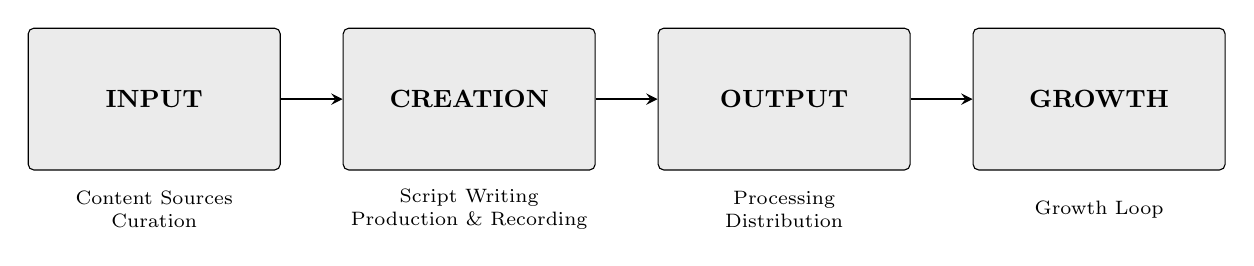
\begin{tikzpicture}[
  stage/.style={draw,rounded corners=2pt,minimum height=1.8cm,minimum width=3.2cm,align=center,font=\small},
  mod/.style={font=\scriptsize,align=center},
  arr/.style={->,thick,>=stealth}
]
  % Stages
  \node[stage,fill=black!8] (input) at (0,0) {\textbf{INPUT}};
  \node[stage,fill=black!8] (creation) at (4,0) {\textbf{CREATION}};
  \node[stage,fill=black!8] (output) at (8,0) {\textbf{OUTPUT}};
  \node[stage,fill=black!8] (growth) at (12,0) {\textbf{GROWTH}};

  % Arrows
  \draw[arr] (input) -- (creation);
  \draw[arr] (creation) -- (output);
  \draw[arr] (output) -- (growth);

  % Modules below
  \node[mod] at (0,-1.4) {Content Sources\\Curation};
  \node[mod] at (4,-1.4) {Script Writing\\Production \& Recording};
  \node[mod] at (8,-1.4) {Processing\\Distribution};
  \node[mod] at (12,-1.4) {Growth Loop};
\end{tikzpicture}
\end{center}
\vspace{0.5em}

We then mapped out \textbf{117 different features} across these 7 modules. Each feature represents a possible capability of the pipeline---from RSS feed ingestion to auto-clipping to comment management.

\subsubsection{FigJam Session with Brett (Meeting \#14)}

We sat down with Brett and walked through all 117 features on a \href{https://www.figma.com/board/qn14Rb37na3RAdAAYPqv7E/Pipeline-Builder-Module-Board}{FigJam board}. For each feature, we discussed what it does and how Brett feels about it. He categorized them into:

\begin{itemize}
  \item \textbf{V0} --- build now (must have for launch)
  \item \textbf{V1} --- build later (next phase)
  \item \textbf{Skip for now} --- not relevant yet
  \item \textbf{Archive} --- interesting but not a priority
\end{itemize}

This gave us a clear understanding of the scope and of what Brett values most. Based on the features he chose or spoke positively about, we defined our V0: \textbf{39 features selected for the first version.}

\subsubsection{Product Backlog}

From the V0 features, we built a structured Product Backlog following the MoSCoW principle:

\begin{itemize}
  \item 39 V0 features, each with Impact/Effort scoring and an owner
  \item Each feature broken into actionable tasks ($\sim$100 total)
  \item Tasks assigned to 4 weekly sprints (Sprint 2--5)
  \item \linkto{https://www.notion.so/Product-Backlog-8304d347036283f7981b819cf684f990}{Product Backlog in Notion}
\end{itemize}

\subsubsection{4-Week Build Plan}
\begin{itemize}
  \item Week 1: Input + Creation start\enspace\textcolor{muted}{|}\enspace Week 2: Creation finish
  \item Week 3: Output\enspace\textcolor{muted}{|}\enspace Week 4: Output + Growth
  \item We are aware this is an ambitious timeline
  \item \linkto{https://b1rd33.github.io/radical-concepts-context/timeline.html}{Interactive Timeline}
\end{itemize}

\subsubsection{Roles}

\smallskip
\renewcommand{\arraystretch}{1.4}
\begin{tabularx}{\textwidth}{@{}l X >{\centering\arraybackslash}p{1.2cm}@{}}
  \arrayrulecolor{border}\toprule
  \textbf{\small Person} & \textbf{\small Responsibility} & \textbf{\small \#} \\
  \midrule
  Chris   & AI prompts, n8n orchestration, infrastructure & 9 \\
  Angelo  & Voice cloning, recording, audio/video processing & 12 \\
  Kalina  & Script review, distribution platforms, style guide & 10 \\
  Roxy    & RSS feeds, curation UX, content source access & 5 \\
  \bottomrule
\end{tabularx}
\renewcommand{\arraystretch}{1}
\arrayrulecolor{black}

\subsubsection{Tools}

We are currently researching tools for each module. These are our current directions---all need further testing before we commit:

\begin{itemize}
  \item \textbf{Orchestration:} n8n as the workflow engine connecting all modules
  \item \textbf{Voice cloning:} For the content-type split (Brett records politics, AI handles science/quirky), getting the emotional tone right is critical. We are looking at Hume AI (recommended by our mentor) for its expressiveness capabilities, alongside ElevenLabs and Fish Audio
  \item \textbf{Auto-clipping:} Opus Pro for extracting the best 60--90\,sec moments from longer recordings
  \item \textbf{Audio cleanup:} Auphonic and Cleanvoice for automated noise removal, filler word removal, and loudness leveling
  \item \textbf{RSS ingestion:} n8n RSS nodes with Jina Reader for full-text extraction
  \item \textbf{Distribution:} Podbean/Castopod for podcast RSS, TubeBuddy for YouTube, Buffer for social
\end{itemize}

\subsubsection{Sprint Workflow}

The Product Backlog is created with 39 features, each containing its own set of tasks. We use a 1-week sprint cadence with 4 sprints remaining until the presentation on April 14. We believe we have finished the brainstorming, ideation, and modularization phase and can now \textbf{focus on building.}

\subsubsection{Research Completed}

We conducted extensive research during Sprint 1, though we have not committed to specific tools yet. Key research includes: competitor landscape analysis (8 competitors), podcast distribution strategy, TTS/voice cloning comparison, Claude prompt templates for news curation and scoring, target audience definition, content format analysis, and monetisation path analysis.

\subsubsection{Design Thinking}
\begin{itemize}
  \item Pain point mapping: 20 Brett + 28 Audience post-its
  \item 6 intersections incl.\ Trust Crisis, Curation IS the Product, Authenticity vs.\ Scale
  \item HMW questions $\rightarrow$ rapid ideation $\rightarrow$ 3 concept directions
  \item \linkto{https://b1rd33.github.io/radical-concepts-context/i2p-brainstorming-board.html}{Interactive Brainstorming Board}
\end{itemize}

% ═══════════════════════════════════════
\section{Stakeholder Feedback}
% ═══════════════════════════════════════

\subsection{Meeting \#8 --- Concept Presentation\enspace\textcolor{muted}{\small Mar 4}}

\begin{feedbackcard}
\begin{itemize}
  \item Appreciated three \textbf{distinct} concepts (not variations)
  \item Strong preference for \textbf{authenticity}---own voice for politics, AI OK for science/quirky
  \item Interested in gamification; skeptical of Dinner Table Drop
  \item Asked to \textbf{refine original podcast concept} with our research
  \item Willing to record 2--3\,min segments: politics 2--3x/week, science 1x/week, quirky 1x/week
  \item Does not want hours rewriting AI scripts
\end{itemize}
\end{feedbackcard}

\subsection{Meeting \#14 --- Pipeline Review\enspace\textcolor{muted}{\small Mar 12}}

\begin{feedbackcard}
\begin{itemize}
  \item Reviewed all 117 features on FigJam; made V0/V1/Archive/Skip decisions per module
  \item Now \textbf{convinced to record himself on video} (initially we explored audio-only with AI avatars)
  \item Wants to \textbf{read articles personally} before script generation---doesn't trust AI to avoid hallucinations
  \item Preferred workflow: pr\'{e}cis $\rightarrow$ read full article $\rightarrow$ ``Generate Script''
  \item \textbf{Hybrid script format}: structured sections with ``Your take here'' prompts for Brett's opinions
  \item Record 3x/week, 25--30\,min; create enough content for the whole week---weekly consistency is key
  \item Opus Pro for auto-clipping; gamification pushed to future community phase
  \item Brett values engagement, confidence, and being upbeat when presenting
\end{itemize}
\end{feedbackcard}

% ═══════════════════════════════════════
\section{Pivots in Priorities}
% ═══════════════════════════════════════

\begin{pivotcard}{3 Concepts \textrightarrow\ 1 Modular Platform}
Brett asked us to refine his original idea rather than pick a new concept. Our research (competitor analysis, audience definition) enriched his existing vision. Result: modular architecture with 7 modules and 117 features enabling incremental delivery.
\end{pivotcard}

\begin{pivotcard}{Audio-Only with AI Avatars \textrightarrow\ Brett on Video}
Initially we explored audio-only content with AI-generated avatars. Through the discussions, Brett became convinced to record himself on video. Video grows audience faster and short-form clips drive discovery on YouTube, TikTok, and Instagram.
\end{pivotcard}

\begin{pivotcard}{Persona-Based Scoring: V1 \textrightarrow\ V0}
Simulating Brett's editorial persona is critical for curation quality. This was initially deprioritized but promoted to V0 after we realized it is the foundation every downstream module depends on. No competitor offers persona-based article scoring.
\end{pivotcard}

\begin{pivotcard}{Full Automation \textrightarrow\ Incremental Quality}
Instead of automating everything and risking credibility, we show Brett individual pieces (script quality, then voice quality, then clip quality). This produces focused, module-level feedback rather than scattered comments on a full demo.
\end{pivotcard}

\begin{pivotcard}{WhatsApp Interface \textrightarrow\ Open Question}
This is not a pivot yet but a question mark. If we send Brett all approvals, scripts, and recording triggers via WhatsApp, it may not be sustainable---too many messages, no overview. We are exploring whether Brett should have a bigger-screen experience (Notion or a simple web dashboard) alongside WhatsApp for quick approvals only.
\end{pivotcard}

\begin{pivotcard}{Content Volume \textrightarrow\ Weekly Batch Recording}
Our priority is that Brett invests the same amount of time he originally planned (about 1--1.5 hours per week) but creates enough content in those sessions to fill the whole week. Weekly consistency matters more than daily recording.
\end{pivotcard}

% ═══════════════════════════════════════
\section{Insights}
% ═══════════════════════════════════════

\begin{insightcard}
\begin{itemize}
  \item \textbf{Don't jump to AI because it's easy.} This is a complex project. It was tempting to start building immediately---AI tools are so accessible that you can have something running in an hour. But following our mentor's advice, we sat down first to think, explore what's out there, and really understand Brett's pain points before writing a single line of automation.

  \item \textbf{Understanding Brett is the real work.} We need to understand his personality, his habits, how much time he's willing to invest, and what will make this feel easy and natural for him---not just technically functional. The design thinking process, the FigJam board, and the pipeline review in Meeting \#14 were invaluable for this.

  \item \textbf{Brett is a filter mechanism himself.} He already has the ability to filter and evaluate news articles. He reads deeply, connects dots across domains, and has strong editorial instincts. The pipeline needs to incorporate and leverage this ability, not replace it. The curation module should amplify his judgment, not automate it away.

  \item \textbf{Fallback mechanisms are a key insight.} If Brett can't record one week, the system should still produce content---through AI-voiced episodes (science/quirky only, never politics), best-of compilations, or newsletter digests. One missed day shouldn't break the habit. This came directly from discussing his recording patterns and lifestyle.

  \item \textbf{The FigJam session shaped our V0.} By walking Brett through 117 features and letting him react to each one, we learned which capabilities he values most. The features he spoke positively about became our V0 scope. This was more effective than us guessing what to prioritize.

  \item \textbf{Build habits, not just tools.} The pipeline needs to fit into Brett's daily routine so naturally that he builds a habit around it. Easy accessibility, minimal friction, predictable structure---these matter more than technical sophistication.
\end{itemize}
\end{insightcard}

% ═══════════════════════════════════════
\section{Links}
% ═══════════════════════════════════════

\renewcommand{\arraystretch}{1.5}
\begin{tabularx}{\textwidth}{@{}>{\small}l >{\small}X@{}}
  \arrayrulecolor{border}\toprule
  \textbf{Deliverable} & \textbf{Link} \\
  \midrule
  Pipeline Builder    & \linkto{https://b1rd33.github.io/radical-concepts-context/pipeline.html}{b1rd33.github.io/.../pipeline.html} \\
  V0 Build Timeline   & \linkto{https://b1rd33.github.io/radical-concepts-context/timeline.html}{b1rd33.github.io/.../timeline.html} \\
  FigJam Board        & \linkto{https://www.figma.com/board/qn14Rb37na3RAdAAYPqv7E/Pipeline-Builder-Module-Board}{FigJam --- Pipeline Module Board} \\
  Concept Pitches     & \linkto{https://b1rd33.github.io/radical-concepts-context/radical-concepts-all-pitches.html}{b1rd33.github.io/.../all-pitches.html} \\
  Design Thinking     & \linkto{https://b1rd33.github.io/radical-concepts-context/i2p-brainstorming-board.html}{b1rd33.github.io/.../brainstorming-board.html} \\
  Product Backlog     & \linkto{https://www.notion.so/Product-Backlog-8304d347036283f7981b819cf684f990}{Notion --- Product Backlog} \\
  GitHub              & \linkto{https://github.com/b1rd33/radical-concepts-context}{github.com/b1rd33/radical-concepts-context} \\
  \bottomrule
\end{tabularx}
\renewcommand{\arraystretch}{1}

\end{document}
